\documentclass[xcolor={table,usenames,dvipsnames}]{beamer}
\usepackage{eso-pic} 
\usepackage[absolute,overlay]{textpos}
\usepackage{colortbl}
\usepackage{fourier}
\usepackage{booktabs}% http://ctan.org/pkg/booktabs
\newcommand{\tabitem}{~~\llap{\textbullet}~~}
\usepackage{tabularx}

\setbeamertemplate{blocks}[rounded][shadow=true]
\let\olditem\item
\renewcommand{\item}{%
\olditem\vspace{-4pt}}     


%\usepackage[round]{natbib} % incompatible avec biblatex
\usepackage{hyperref}
\hypersetup{
    colorlinks=true,
    linkcolor=.,
    filecolor=magenta,      
    urlcolor=deepblue,
    pdftitle={Overleaf Example},
    pdfpagemode=FullScreen,
    citecolor=deepblue
    }
\definecolor{LightCyan}{rgb}{0.88,1,1}   
\usepackage[justification=centering]{caption}
\captionsetup{font=scriptsize}
\captionsetup[figure]{name=Fig.}
\setbeamertemplate{caption}[numbered]
\usepackage[T1]{fontenc}
\usepackage{ctex}
\UseRawInputEncoding
\usepackage[backend=bibtex,
style=authoryear,
natbib=true,
sorting=nty,
backref=true
]{biblatex}
\renewcommand*{\bibfont}{\footnotesize}

\DeclareCiteCommand{\cite}
  {\usebibmacro{prenote}}
  {\usebibmacro{citeindex}%
   \printtext[bibhyperref]{\usebibmacro{cite}}}
  {\multicitedelim}
  {\usebibmacro{postnote}}

\DeclareCiteCommand*{\cite}
  {\usebibmacro{prenote}}
  {\usebibmacro{citeindex}%
   \printtext[bibhyperref]{\usebibmacro{citeyear}}}
  {\multicitedelim}
  {\usebibmacro{postnote}}

\DeclareCiteCommand{\parencite}[\mkbibparens]
  {\usebibmacro{prenote}}
  {\usebibmacro{citeindex}%
    \printtext[bibhyperref]{\usebibmacro{cite}}}
  {\multicitedelim}
  {\usebibmacro{postnote}}

\DeclareCiteCommand*{\parencite}[\mkbibparens]
  {\usebibmacro{prenote}}
  {\usebibmacro{citeindex}%
    \printtext[bibhyperref]{\usebibmacro{citeyear}}}
  {\multicitedelim}
  {\usebibmacro{postnote}}

\DeclareCiteCommand{\footcite}[\mkbibfootnote]
  {\usebibmacro{prenote}}
  {\usebibmacro{citeindex}%
  \printtext[bibhyperref]{ \usebibmacro{cite}}}
  {\multicitedelim}
  {\usebibmacro{postnote}}

\DeclareCiteCommand{\footcitetext}[\mkbibfootnotetext]
  {\usebibmacro{prenote}}
  {\usebibmacro{citeindex}%
   \printtext[bibhyperref]{\usebibmacro{cite}}}
  {\multicitedelim}
  {\usebibmacro{postnote}}

%\DeclareCiteCommand{\textcite}
%  {\boolfalse{cbx:parens}}
%  {\usebibmacro{citeindex}%
%   \printtext[bibhyperref]{\usebibmacro{textcite}}}
%  {\ifbool{cbx:parens}
%     {\bibcloseparen\global\boolfalse{cbx:parens}}
%     {}%
%   \multicitedelim}
%  {\usebibmacro{textcite:postnote}}

        \DeclareCiteCommand{\textcite}
        {\usebibmacro{cite:init}%
            \usebibmacro{prenote}}
        {\usebibmacro{citeindex}%
            \printtext[bibhyperref]{\usebibmacro{textcite}}}
        {}
        {\printtext[bibhyperref]{\usebibmacro{textcite:postnote}}%
            \usebibmacro{cite:post}}

\addbibresource{ref.bib}

% Cannot enable in Xelatex
\usepackage{pgfpages}
% \setbeameroption{hide notes} % Only slides
% \setbeameroption{show only notes} % Only notes
% \setbeameroption{show notes on second screen}

% other packages
\usepackage{latexsym,amsmath,multicol,booktabs,calligra}
\usepackage{graphicx,listings,stackengine}
\usepackage[french]{babel}
\DefineBibliographyStrings{french}{%
  backrefpage = {voir p\adddot},%
  backrefpages = {voir pp\adddot}%
}
\DeclareFieldFormat{pagerefformat}{\mkbibparens{{\color{red}\mkbibemph{#1}}}}
\renewbibmacro*{pageref}{%
  \iflistundef{pageref}
    {}
    {\printtext[pagerefformat]{%
       \ifnumgreater{\value{pageref}}{1}
         {\bibstring{backrefpages}\ppspace}
         {\bibstring{backrefpage}\ppspace}%
       \printlist[pageref][-\value{listtotal}]{pageref}}}}
\usepackage{wasysym}
% Enable only in Xelatex
 \usepackage{pstricks}

\author[Lj. PETKOVIC \textit{et al.}]{\small \textbf{Ljudmila PETKOVIC}\textsuperscript{1,2,3}, Motasem ALRAHABI\textsuperscript{1,3}, Glenn ROE\textsuperscript{1,2,3}\\\medskip{\texttt{prenom.nom@sorbonne-universite.fr}}}
\title[Dans les petits papiers de Charcot$\dots$]{\fontsize{13pt}{13pt}\selectfont Dans les petits papiers de Charcot :}
\subtitle{de l’expérimentation aux prémisses de la neurologie moderne}
\institute [JE \og{}Humanités numériques\fg{}] {\tiny \textsuperscript{1} Sorbonne Université, Faculté des Lettres, \textsc{UFR} Littératures françaises et comparée\\\textsuperscript{2} Centre d'étude de la langue et des littératures françaises (\textsc{CELLF}), \textsc{UMR 8599}\\\textsuperscript{3} Observatoire des textes, des idées et des corpus (\textsc{ObTIC})}
\date[\today]{\scriptsize  Séminaire doctoral du \textsc{CERES}\\Maison de la Recherche, Sorbonne Université\\Paris, \today}
\usepackage{YTU}

% defs
\def\cmd#1{\texttt{\color{red}\footnotesize $\backslash$#1}}
\def\env#1{\texttt{\color{blue}\footnotesize #1}}
\definecolor{deepblue}{rgb}{0,0,0.5}
\definecolor{deepred}{rgb}{0.6,0,0}
\definecolor{deepgreen}{rgb}{0,0.5,0}
\definecolor{halfgray}{gray}{0.55}

\lstset{
    basicstyle=\ttfamily\small,
    keywordstyle=\bfseries\color{deepblue},
    emphstyle=\ttfamily\color{deepred},    % Custom highlighting style
    stringstyle=\color{deepgreen},
    numbers=left,
    numberstyle=\small\color{halfgray},
    rulesepcolor=\color{red!20!green!20!blue!20},
    frame=shadowbox,
}
% \logo{%
%     
\includegraphics[width=1cm,height=1cm,keepaspectratio]{pic/obtic.jpg}~%
%     
\includegraphics[width=1cm,height=1cm,keepaspectratio]{pic/Lettres_su_logo.png}~%
% }

\setbeamertemplate{section in toc}{\hspace*{1em}\inserttocsectionnumber.~\inserttocsection\par}
\setbeamertemplate{subsection in toc}{\hspace*{2em}\inserttocsectionnumber.\inserttocsubsectionnumber.~\inserttocsubsection\par}
\renewcommand*{\bibfont}{\scriptsize}

\setbeamertemplate{itemize/enumerate body begin}{\small}
\setbeamertemplate{itemize/enumerate subbody begin}{\footnotesize}

\let\oldfootnotesize\footnotesize
\renewcommand*{\footnotesize}{\oldfootnotesize\scriptsize}



\begin{document}

\begin{frame}
    \titlepage
\begin{figure}
    \centering
    
    
\includegraphics[width=2cm,height=1cm,keepaspectratio]{pic/Lettres_su_logo.png}~\hspace*{0.5cm}%\includegraphics{}
    
\includegraphics[width=2cm,height=1cm,keepaspectratio]{pic/cellf.png}~\hspace*{0.5cm}%
    
\includegraphics[width=3cm,height=1cm,keepaspectratio]{pic/obtic.jpg}~%

\end{figure}
    
    \begin{note}
        {Introduce your self}
    \end{note}

\end{frame}

\begin{frame}
\frametitle{Plan}
    \tableofcontents[sectionstyle=show,subsectionstyle=show,subsubsectionstyle=show/shaded/hide]
\end{frame}

\section[Contexte]{Contexte de recherche}
%\subsection{Rupture épistémologique}
\begin{frame}{Le progrès de la science comme un processus discontinu}
\begin{block}{Rupture épistémologique}
Passage radical d'un paradigme\footnote{découverte scientifique universellement reconnue.} à un autre, dans la façon dont les scientifiques abordent un domaine donné.
\end{block}
\begin{itemize}
\small
\item \og{}rupture entre observation et expérimentation \fg{}
{\footnotesize(\cite{bachelard1934formation})}
\item \og{}révolution scientifique\fg{} {\footnotesize(\cite{koyre1957closed})}
\item \og{}changement de paradigme\fg{} {\footnotesize(\cite{kuhn1962structure})} 
\end{itemize} 
%Le nouveau paradigme est incompatible avec le précédent, p. ex. géo- \textit{vs.} héliocentrisme.
\begin{minipage}{5cm}
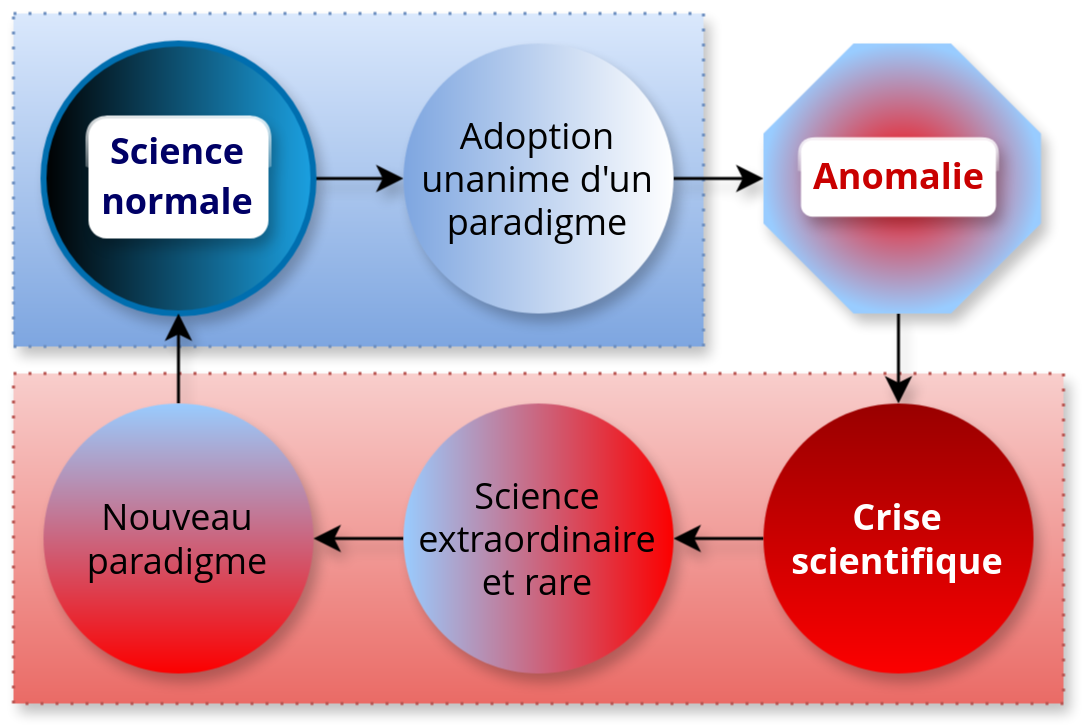
\includegraphics[height=3cm, width=4.5cm]{pic/changement_paradigme.png}
\end{minipage}%
\begin{minipage}{6cm}
{\normaltext Conception kuhnienne du progrès scientifique, adaptée de {\small\textcite{amiri}}}. \bigskip

 {\scriptsize Le nouveau paradigme est incompatible avec le précédent, p. ex. géo- \textit{vs.} héliocentrisme.}
\end{minipage}
%\begin{figure}
%    \centering
%    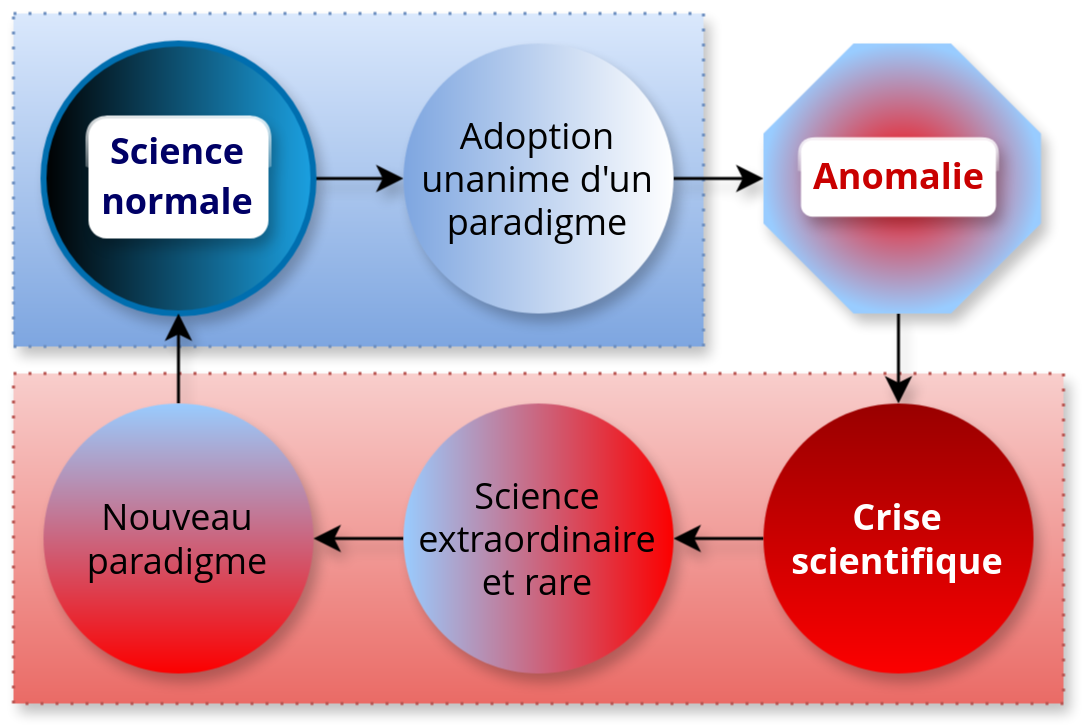
\includegraphics[width=65mm,scale=0.5]{pic/changement_paradigme.png}
%    \caption{Conception kuhnienne du progrès scientifique, adaptée de {\scriptsize\textcite{amiri}}.}
%    \label{fig:enter-label}
%\end{figure}
\end{frame}


%\subsection{Évolution du terme \textit{hystérie}}
%\begin{frame}{Évolution du terme \textit{hystérie}}
Exemple du changement de paradigme : le terme d'\textsc{hystérie}
\begin{itemize}
 \item grec \textgreek{ὑστέρα}, latin \textit{hystera} : \og{}utérus, matrice\fg{} 
\end{itemize}
\begin{table}[h!]
\footnotesize
\begin{tabular}{lcl}
\multicolumn{1}{l}{\textrm{Période}} & \multicolumn{1}{c}{\textrm{Sexe}} & \multicolumn{1}{c}{\textrm{Étiologie}}   \\
\hline \hline
Antiquité   & \female{}             & \begin{tabular}[c]{@{}l@{}}{\footnotesize déplacement de l'utérus, selon Hippocrate \citep{tasca2012women}
%\footnote{{\footnotesize\cite{tasca2012women}}}
\\\textit{hystérique} : (femme) malade de l'utérus}\end{tabular}          \\ \hline
Moyen Âge   & \female{}             & \begin{tabular}[c]{@{}l@{}}{\footnotesize possession démoniaque, superstition religieuse de l'Église
%\footnote{{\footnotesize\cite{tasca2012women}}}
\\ 	$\rightarrow$ chasses, tortures, exorcismes \citep{tasca2012women}}\end{tabular} \\ \hline
Renaissance & \female{}/\male{}           & \begin{tabular}[c]{@{}l@{}}{\footnotesize localisation dans le cerveau, \textit{sensorium commune} \citep{lepois1618}
%\footnote{{\footnotesize\cite{lepois1618}}}
\\\og{}siège commun de la sensibilité\fg{}\footnote{\cite{kant1863}.}, ensemble des perceptions}\end{tabular}   \\ \hline
Lumières    & \female{}/\male{}           & \begin{tabular}[c]{@{}l@{}}{\footnotesize explosion des \og{}esprits animaux\fg{} dans le cerveau\\maladie convulsive \citep{willispathologiae}\footnote{{\footnotesize créateur du terme \textit{neurologia} en 1664.}}}\end{tabular} \\ \hline
\rowcolor{LightCyan}
\textsc{XIX}\ieme{} s. & \female{}/\male{} & \begin{tabular}[c]{@{}l@{}}{\footnotesize dégénérescence héréditaire du système nerveux \citep{charcot1870}
%\footnote{{\footnotesize\cite{charcot1870}}}
\\maladie systématiquement traitée comme un trouble neurologique}
\end{tabular}
\end{tabular}
\end{table}
\begin{itemize}
\end{itemize}
\end{frame}





%\subsection{\og Napoléon des névroses \fg{} ou \og Paganini de l'hystérie \fg{}  }
%\begin{frame}{\og{}Napoléon des névroses \fg{} ou \og{}Paganini de l’hystérie\fg{} {\small(\hypersetup{citecolor=yellow}\cite{marmion2015freud})}}

{\textsc{Jean-Martin Charcot (1825-1893)}}
%\hbox{\hspace{25em} 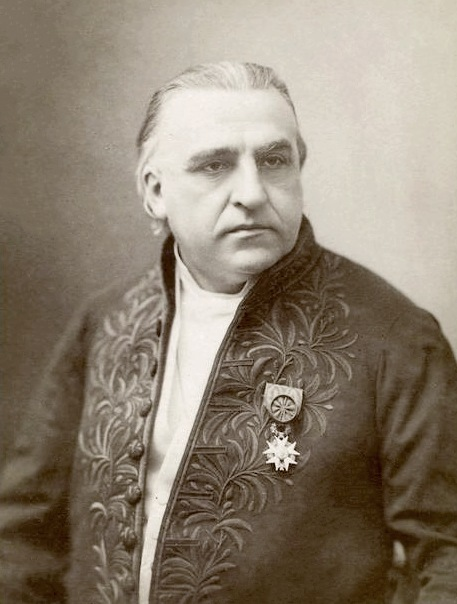
\includegraphics[scale=0.07]{pic/Jean-Martin_Charcot.jpg}}
%\\{\scriptsize Portrait de\\Charcot (\href{https://fr.wikipedia.org/wiki/Jean-Martin_Charcot}{Wikipedia}).}
\hbox{\hspace{6em} 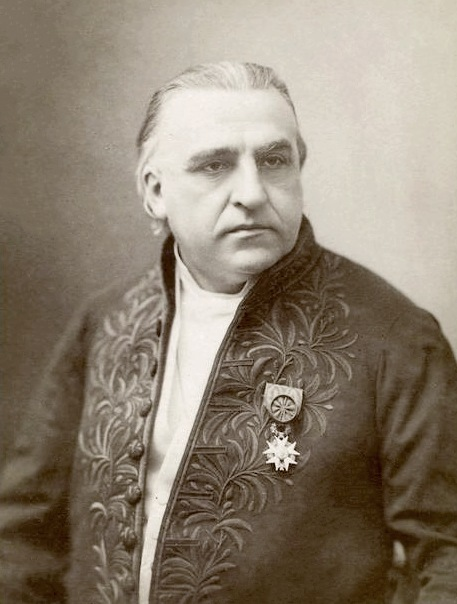
\includegraphics[scale=0.08]{pic/Jean-Martin_Charcot.jpg}}\\\hbox{\hspace{23.3em}{\tiny Source : \href{https://fr.wikipedia.org/wiki/Jean-Martin_Charcot}{Wikipedia}}.}
\begin{itemize}
\item père de la neurologie moderne au XIX\ieme{} s. 
\item leçons cliniques du mardi à l'hôpital de la Salpêtrière à Paris 
\end{itemize}
\begin{itemize}
	\item[] Contributions majeures :
	\begin{itemize}
	    \item hystérie : résultat d'une lésion dynamique des circuits cérébraux
    \item hypnose : outil thérapeutique pour les hystériques
    \item SEP\footnote{abbr. \textit{sclérose en plaques}.} disséminée (description) $\rightarrow$ sclérose multiple
    \item SLA\footnote{abbr. \textit{sclérose latérale amyotrophique}.} (description) $\rightarrow$ maladie de Charcot / Lou Gehrig
    \item maladie de Parkinson : concepteur du terme (avec A. Vulpian)
	\end{itemize}
	\end{itemize}
    
    % \item hystérie est due à une \textit{lésion dynamique} de l’encéphale, liée à un traumatisme de nature physique (accident de train, chute, choc$\dots$) -- possible de recréer sous hypnose

    % \item impact sur les acteurs dans ou en dehors de sa discipline : S. Freud, G. de la Tourette, E. Zola$\dots$

{\footnotesize(\cite{teive2022thomas})}

%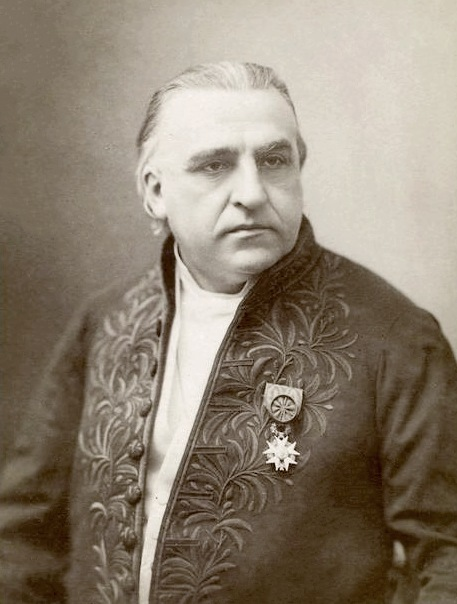
\includegraphics[width=10pt]{pic/Jean-Martin_Charcot.jpg}%
%\\{\scriptsize Portrait de\\Charcot (\href{https://fr.wikipedia.org/wiki/Jean-Martin_Charcot}{Wikipedia}).}



\end{frame}



\section[Objectifs]{Problématique et objectifs}
%\subsection{Impact de Charcot sur son réseau scientifique et artistique}
%\begin{frame}{Impact de Charcot sur sa discipline et au-delà}
\textbf{Collaborateurs et élèves}
\centering
    \begin{table}[!ht]
        \centering
        \small
        \begin{tabular}{l r}
           Sigmund \textsc{Freud} (1856-1939)  & théorie psychanalytique \\
            Gilles \textsc{de la Tourette} (1857-1932) & syndrôme de Tourette \\
            Joseph \textsc{Babinski} (1857-1904) & pithiatisme, signe de Babinski \\
            Pierre \textsc{Janet} (1859-1947) & dissociation, sous-conscient 
        \end{tabular}
        \begin{flushright}
        \footnotesize\citep{bogousslavsky2020}
        \end{flushright}
        % \caption{Caption}
        \label{tab:my_label}
    \end{table}
\medskip
\textbf{Littéraires} 
\begin{itemize}
\item références à Charcot et descriptions de crises hystériques dans la littérature naturaliste française et européenne
\end{itemize}
\begin{table}[!ht]
    \centering
    \small
    \begin{tabular}{l r}
        Émile \textsc{Zola} (1840–1902)  & \textit{Lourdes} \\
        Léon \textsc{Tolstoï} (1828–1910) & \textit{La Sonate à Kreutzer} \\
        Luigi \textsc{Capuana} (1839–1915) & \textit{La Torture} \\
        Bjørnstjerne \textsc{Bjørnson} (1832–1910) & \textit{Over Ævne}
    \end{tabular}
            \begin{flushright}
        \footnotesize\citep{koehler2013charcot}
        \end{flushright}
    % \caption{Caption}
    \label{tab:my_label}
\end{table}

\end{frame}


%
%\subsection{Circulation du discours médical au prisme du numérique}
%\begin{frame}{Circulation du discours médical au prisme du numérique}
\centering
Objectif : aborder computationnellement la question des circulations des phénomènes textuels complexes.
\begin{figure}
    \centering
    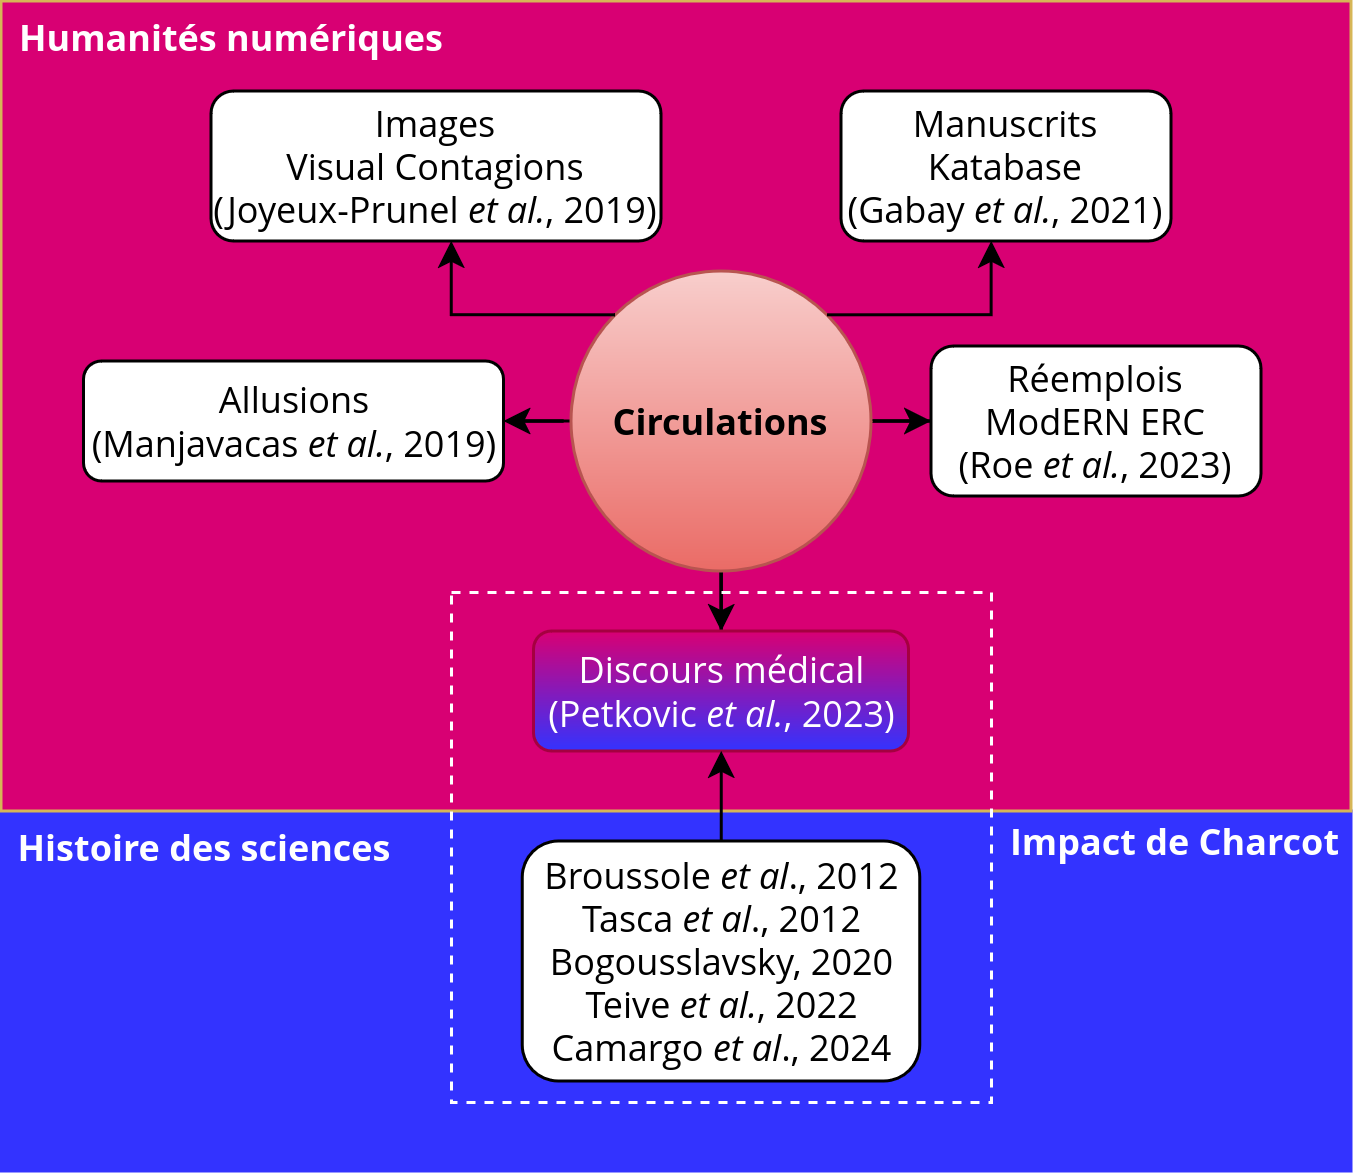
\includegraphics[width=65mm,scale=0.5]{pic/dh_histoire-sciences.png}
    \caption{Études (numériques) des circulations des savoirs.}
    \label{fig:enter-label}
\end{figure}
\notecite{joyeux2019visual}
\notecite{gabay2021katabase}
\notecite{manjavacas2019}
\notecite{tasca2012women}
\notecite{bogousslavsky2020}
\nocite{camargo2024}
% Influence de Charcot : \cite{bogousslavsky}, \cite{camargo}
% Constitution et exploitation de ce fonds au prisme du numérique
\end{frame}



%\subsection{Question de recherche}
%\begin{frame}{Question de recherche}
% Comment mesurer le degré d'intertextualité entre Charcot et son réseau scientifique et artistique au prisme du numérique ?
% create the main block
\begin{exampleblock}{}
    \color{deepblue}{\textmd{Comment mesurer le degré d'intertextualité entre Charcot et son réseau scientifique et/ou artistique au prisme du numérique ?}}
\end{exampleblock}

\end{frame}


\section[Méthodologie]{Méthodologie de recherche}
%\subsection{Fonds Charcot}
%\begin{frame}{Fonds Charcot}
\begin{block}{SorbonNum\footnote{\tiny{\url{https://patrimoine.sorbonne-universite.fr/}}} -- Bibliothèque de Sorbonne Université (BSU)}
201 documents XML OCRisés (sans post-correction)
\end{block}
\begin{itemize}
    \item \textrm{Charcot} : textes rédigés par Charcot et ses collègues
    \item \textrm{Autres} : textes rédigés par ses collègues
\end{itemize}
\begin{table}[!ht]
    \centering
    \begin{tabular}{|c|c|c|}
    \hline 
    \rowcolor{gray!30}
       Corpus & Nb de docs & Nb de tokens \\
       \hline
       \textrm{Charcot}  & 68 & 12 190 649 (38,12\%) \\
       \textrm{Autres}  & 133 & 19 788 830 (61,88\%) \\
       \hline\hline
       \textbf{Total} & \textbf{201} & \textbf{31 979 479} (100\%)\\
       \hline
    \end{tabular}
    \caption{Répartition du corpus issu du fonds Charcot\footnote{\tiny{\url{https://patrimoine.sorbonne-universite.fr/collection/Fonds-Charcot}}}.}
    \label{tab:my_label}
\end{table}
\end{frame}

%\subsection{Mesurer le degré d'intertextualité}
%\begin{frame}{Mesurer le degré d'intertextualité}

{\small(\textit{Traductologie}) Mesurer l'influence d'un écrivain sur le style de son traducteur {\footnotesize(\cite{oseki2007})}.}
\begin{itemize}
\item[$\rightarrow$] mesurer informatiquement l'impact de Charcot sur son réseau : intertextualité uni-directionnelle
\end{itemize}
\begin{figure}[!h]
    \centering
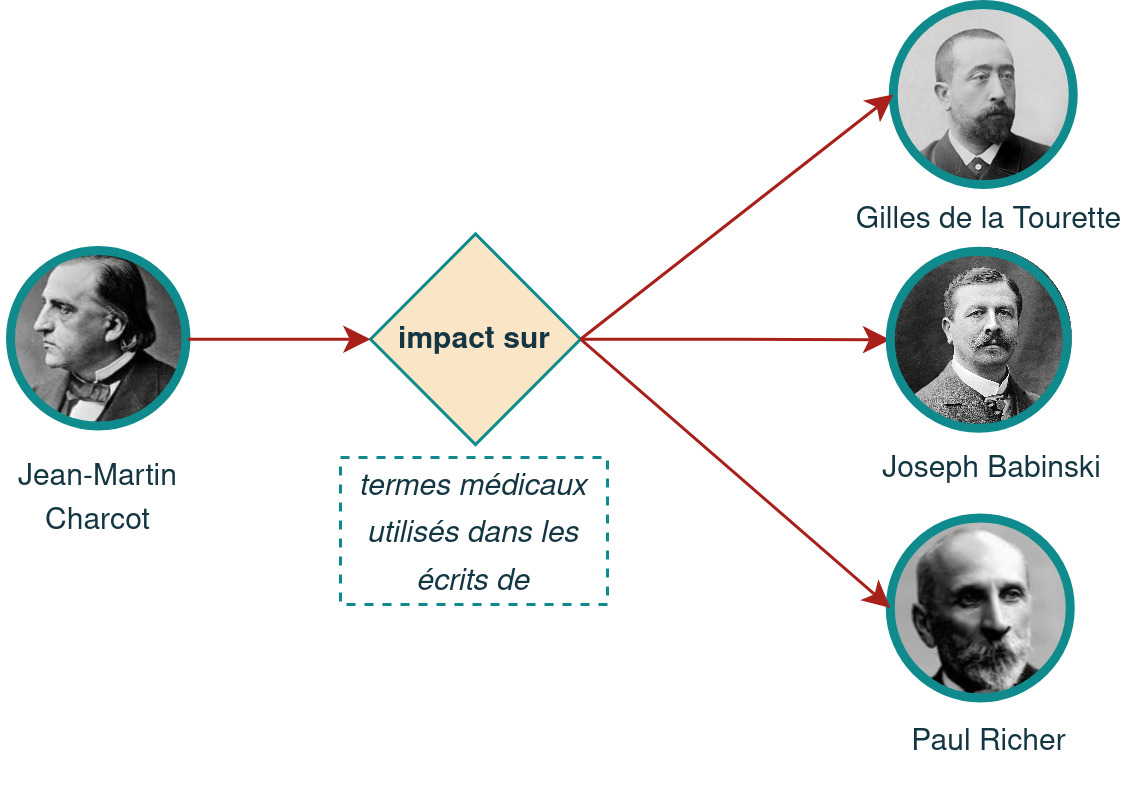
\includegraphics[width=65mm,scale=0.5]{pic/charcot_intertextualite.jpg}
    \caption{Opérationnalisation de l'impact de Charcot sur ses élèves.}
    \label{fig:my_label}
\end{figure}
\end{frame}



%\subsection{Premières analyses du corpus Charcot}
%\begin{frame}{Première analyse du corpus Charcot}
\color{deepblue}{OBVIE\footnote{\url{https://obtic.huma-num.fr/obvie/}}}
\begin{itemize}
    \item moteur de recherche pour la fouille avancée des corpus en \textsc{XML-TEI}
    \item identification des substantifs les plus importants 
    \begin{itemize}
        \item fréquences brutes, mesures \textsc{TF-IDF}, \textsc{BM25}, $\chi^2$, Test Gamma
    \end{itemize}
    \item repérage des textes similaires par ordre de pertinence
    \begin{itemize}
    \item à partir des termes en commun et termes fréquents
\end{itemize}     
\end{itemize}
\end{frame}



\begin{frame}{Deuxième analyse du corpus Charcot}
    \color{deepblue}{TextPair\footnote{\scriptsize\url{https://artfl-project.uchicago.edu/text-pair}}}
    \begin{itemize}
        \item aligne des passages similaires dans une collection de textes
        \begin{itemize}
        \item passages incluant des citations, plagiats, emprunts, réemplois$\dots$
        \end{itemize}
        \item génère une liste de séquences similaires pour chaque texte
        \begin{itemize}
        \item séquences de mots qui se chevauchent (trigrammes de mots)
        \end{itemize}        
        \item compare les séquences générées du texte \textit{source} au texte \textit{cible}
    \end{itemize}
\end{frame}




%\subsection{Calcul de pertinence des concepts médicaux}
%%\begin{frame}{Notre approche}
%Repérage des concepts dans les deux corpus en se basant sur le poids de leur apparition
%\begin{table}[!ht]
%\footnotesize
%\begin{tabularx}{\textwidth}{>{\setlength\hsize{1\hsize}\setlength\linewidth{\hsize}}X>{\setlength\hsize{1\hsize}\setlength\linewidth{\hsize}}X>{\setlength\hsize{1\hsize}\setlength\linewidth{\hsize}}X}
%\hline
%\rowcolor{blue!10}
%\multicolumn{3}{c}{Mesures de pondération}\\
%\textsc{TF-IDF} & \textsc{BM25} & \textsc{BERT} \\
%\hline
%\begin{itemize}
%    \item évalue l’importance d’un terme contenu dans
%un document relativement à un corpus plus
%large 
%    \item récompense la fréquence des
%termes et pénalise la fréquence des documents 
%\end{itemize}
%
%&
%\begin{itemize}
%    \item amélioration de \textsc{TF-IDF} 
%    \item traite les longs documents et les problèmes liés à la saturation des termes
%\end{itemize}
% &
% \begin{itemize}
%     \item modèle pré-entraîné sur de gros corpus (apprentissage non-supervisé, architecture des transformeurs)
%     \item apprend des représentations de mots et de phrases (contexte + sémantique)
%     % \item architecture des transformeurs (réseau de neurones utilisé pour le TAL)
% \end{itemize}
%\end{tabularx}
%\end{table}
%\end{frame}

\begin{frame}{Liste des concepts médicaux}
    Extraction des termes ou des expressions popularisés par Charcot (\textit{hystérie}, \textit{sclérose latérale amyotrophique} etc.)
    \begin{itemize}
        \item index d’une édition des œuvres complètes de Charcot\footnote{\cite{charcot1890oeuvres}}
        \item sans les termes génériques (\textit{os, \textit{cerveau}, etc.})
        \item prise en compte des formes singulier / pluriel (regex)
    \end{itemize}
\end{frame}

\begin{frame}{Intensification du lexique
de Charcot dans le corpus \og{}Autres\fg}
\begin{figure}[!h]
    \centering
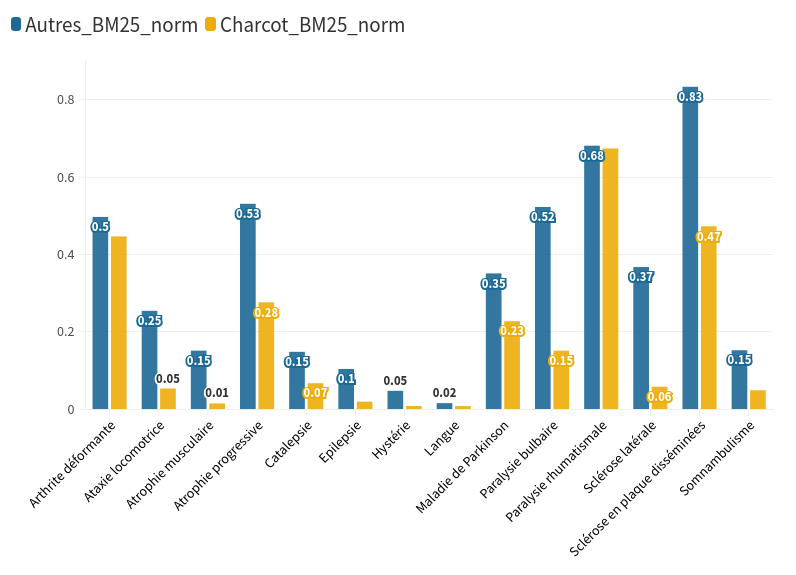
\includegraphics[width=94mm,scale=0.5]{pic/Charcot_Autres_250523.png}
    \caption{Pertinence des concepts dans les deux corpus (BM25).}
    \label{fig:my_label}
\end{figure}
\end{frame}

\begin{frame}{\textsc{TF-IDF}}
(angl. \textit{term frequency-inverse document frequency})\medskip

\color{deepblue}
Mesure pour quantifier l'importance ou la pertinence des représentations lexicales (mots, phrases, lemmes$\dots$) dans un document parmi une collection de documents (corpus).
\begin{itemize}
\item \textbf{TF} : fréquence d'un terme particulier par rapport au document.
\item \textbf{IDF} : calcule à quel point un terme est courant (ou rare) dans le corpus
\begin{itemize}
\item pénalise des termes fréquents et récompense les termes peu fréquents (considérés comme plus discriminants)
\end{itemize}
\end{itemize}
\end{frame}

\begin{frame}{\textsc{BM-25}}
(angl. \textit{best match} 25)\medskip

\color{deepblue}{Modèle de classement basé sur des termes qui vise à fournir des résultats de recherche précis et pertinents en classant les documents en fonction de la fréquence de leurs termes et de leur longueur.}

\begin{enumerate}
\item TF
\item IDF
\item normalisation de la longueur des documents
\item saturation des termes de requête
\end{enumerate}
\medskip

\color{deepgreen}{TF-IDF et BM25 sont les mesures couramment utilisées dans le domaine de recherche d'information (angl. \textit{information retrieval})}

\end{frame}

\begin{frame}{\textsc{BERT}}
\cite{vaswani2021}
    \begin{itemize}
        \item plongements lexicaux et des
mécanismes d’attention
        \item modèle \texttt{bert-base-multilingual-cased}
    \end{itemize}

\begin{table}[]
\begin{tabular}{ll}
\hline
Corpus « Charcot »             & Corpus « Autres » \\
\hline
diplopie (0,92)                & préambule (0,47)  \\
myélite partielle (0,91)       & délire (0,47)     \\
état de mal épileptique (0,91) & miracle (0,47)   \\
paralysie labio-glosso-laryngée (0,91) &
cicatrices vicieuses (0,46) \\
\textsc{pathologies} & \textsc{notions abstraites} \\
\hline 
\end{tabular}
\end{table}
\end{frame}

\begin{frame}{Calcul de pertinence des concepts I}
\footnotesize
\begin{table}[]
\begin{tabular}{|l|cccc|}
\hline
\multicolumn{1}{|c|}{{ }} &
  \multicolumn{4}{c|}{\cellcolor[HTML]{FCFF2F}{ Corpus \og{}Charcot\fg{}}} \\ \cline{2-5} 
\multicolumn{1}{|c|}{\multirow{}{}{{ Terme}}} &
  {Fréquence} &
  {TF-IDF} &
  {BM25} &
  {BERT} \\ \hline
{Arthrite déformante} &
  \multicolumn{1}{|c|}{{30}} &
  \multicolumn{1}{|c|}{{0,16}} &
  \multicolumn{1}{|c|}{{0,45}} &
  {0,80} \\ \hline
{Ataxie locomotrice} &
  \multicolumn{1}{|c|}{{559}} &
  \multicolumn{1}{|c|}{{0,35}} &
  \multicolumn{1}{|c|}{{0,05}} &
  {0,83} \\ \hline
{Atrophie musculaire} &
  \multicolumn{1}{|c|}{{1105}} &
  \multicolumn{1}{|c|}{{0,20}} &
  \multicolumn{1}{|c|}{{0,02}} &
  {0,84} \\ \hline
{Atrophie progressive} &
  \multicolumn{1}{|c|}{{40}} &
  \multicolumn{1}{|c|}{{0,14}} &
  \multicolumn{1}{|c|}{{0,27}} &
  {0,72} \\ \hline
{Catalepsie} &
  \multicolumn{1}{|c|}{{681}} &
  \multicolumn{1}{|c|}{{0,54}} &
  \multicolumn{1}{|c|}{{0,07}} &
  {0,88} \\ \hline
{Épilepsie} &
  \multicolumn{1}{|c|}{{414}} &
  \multicolumn{1}{|c|}{{0,09}} &
  \multicolumn{1}{|c|}{{0,02}} &
  {0,78} \\ \hline
{Hystérie} &
  \multicolumn{1}{|c|}{{5775}} &
  \multicolumn{1}{|c|}{{0,51}} &
  \multicolumn{1}{|c|}{{0,01}} &
  {0,74} \\ \hline
{Langue} &
  \multicolumn{1}{|c|}{{2695}} &
  \multicolumn{1}{|c|}{{0,24}} &
  \multicolumn{1}{|c|}{{0,01}} &
  {0,72} \\ \hline
{Maladie de Parkinson} &
  \multicolumn{1}{|c|}{{75}} &
  \multicolumn{1}{|c|}{{0,21}} &
  \multicolumn{1}{|c|}{{0,23}} &
  {0,81} \\ \hline
{Paralysie bulbaire} &
  \multicolumn{1}{|c|}{{149}} &
  \multicolumn{1}{|c|}{{0,27}} &
  \multicolumn{1}{|c|}{{0,15}} &
  {0,89} \\ \hline
{Paralysie rhumatismale} &
  \multicolumn{1}{|c|}{{8}} &
  \multicolumn{1}{|c|}{{0,07}} &
  \multicolumn{1}{|c|}{{0,67}} &
  {0,86} \\ \hline
{Sclérose latérale} &
  \multicolumn{1}{|c|}{{445}} &
  \multicolumn{1}{|c|}{{0,30}} &
  \multicolumn{1}{|c|}{{0,06}} &
  {0,88} \\ \hline
{Sclérose en plaque disséminées} &
  \multicolumn{1}{|c|}{{45}} &
  \multicolumn{1}{|c|}{{0,25}} &
  \multicolumn{1}{|c|}{{0,47}} &
  {0,87} \\ \hline
{Somnambulisme} &
  \multicolumn{1}{|c|}{{847}} &
  \multicolumn{1}{|c|}{{0,49}} &
  \multicolumn{1}{|c|}{{0,05}} &
  {0,89} \\ \hline
\end{tabular}
\caption{Calcul de pertinence des concepts selon les mesures TF-IDF, BM25 et BERT dans le corpus \og{}Charcot\fg{}.}
\end{table}
\end{frame}

\begin{frame}{Calcul de pertinence des concepts II}
    \footnotesize
\begin{table}[]
\begin{tabular}{|l|cccc|}
\hline
\multicolumn{1}{|c|}{{ }} &
  \multicolumn{4}{c|}{\cellcolor[HTML]{DAE8FC}{ Corpus \og{}Autres\fg{}}} \\ \cline{2-5} 
\multicolumn{1}{|c|}{\multirow{}{}{{ Terme}}} &
  {Fréquence} &
  {TF-IDF} &
  {BM25} &
  {BERT} \\ \hline
{Arthrite déformante} &
  \multicolumn{1}{|c|}{{24}} &
  \multicolumn{1}{|c|}{{0,02}} &
  \multicolumn{1}{|c|}{{\textbf{0,50}}} &
  {0,40} \\ \hline
{Ataxie locomotrice} &
  \multicolumn{1}{|c|}{{169}} &
  \multicolumn{1}{|c|}{{0,08}} &
  \multicolumn{1}{|c|}{{0,25}} &
  {0,39} \\ \hline
{Atrophie musculaire} &
  \multicolumn{1}{|c|}{{1465}} &
  \multicolumn{1}{|c|}{{0,43}} &
  \multicolumn{1}{|c|}{{0,15}} &
  {0,42} \\ \hline
{Atrophie progressive} &
  \multicolumn{1}{|c|}{{22}} &
  \multicolumn{1}{|c|}{{0,02}} &
  \multicolumn{1}{|c|}{{0,53}} &
  {0,39} \\ \hline
{Catalepsie} &
  \multicolumn{1}{|c|}{{975}} &
  \multicolumn{1}{|c|}{{0,28}} &
  \multicolumn{1}{|c|}{{0,15}} &
  {0,39} \\ \hline
{Épilepsie} &
  \multicolumn{1}{|c|}{{577}} &
  \multicolumn{1}{|c|}{{0,12}} &
  \multicolumn{1}{|c|}{{0,10}} &
  {0,41} \\ \hline
{Hystérie} &
  \multicolumn{1}{|c|}{{4934}} &
  \multicolumn{1}{|c|}{{0,45}} &
  \multicolumn{1}{|c|}{{0,05}} &
  {0,41} \\ \hline
{Langue} &
  \multicolumn{1}{|c|}{{3591}} &
  \multicolumn{1}{|c|}{{0,11}} &
  \multicolumn{1}{|c|}{{0,02}} &
  {0,41} \\ \hline
{Maladie de Parkinson} &
  \multicolumn{1}{|c|}{{130}} &
  \multicolumn{1}{|c|}{{0,09}} &
  \multicolumn{1}{|c|}{{0,35}} &
  {0,37} \\ \hline
{Paralysie bulbaire} &
  \multicolumn{1}{|c|}{{93}} &
  \multicolumn{1}{|c|}{{0,09}} &
  \multicolumn{1}{|c|}{{0,52}} &
  {0,40} \\ \hline
{Paralysie rhumatismale} &
  \multicolumn{1}{|c|}{{14}} &
  \multicolumn{1}{|c|}{{0,02}} &
  \multicolumn{1}{|c|}{{\textbf{0,68}}} &
  {0,44} \\ \hline
{Sclérose latérale} &
  \multicolumn{1}{|c|}{{127}} &
  \multicolumn{1}{|c|}{{0,09}} &
  \multicolumn{1}{|c|}{{0,37}} &
  {0,41} \\ \hline
{Sclérose en plaque disséminées} &
  \multicolumn{1}{|c|}{{12}} &
  \multicolumn{1}{|c|}{{0,02}} &
  \multicolumn{1}{|c|}{{\textbf{0,83}}} &
  {0,40} \\ \hline
{Somnambulisme} &
  \multicolumn{1}{|c|}{{3410}} &
  \multicolumn{1}{|c|}{{1}} &
  \multicolumn{1}{|c|}{{0,15}} &
  {0,43} \\ \hline
\end{tabular}
\caption{Calcul de pertinence des concepts selon les mesures TF-IDF, BM25 et BERT dans le corpus \og{}Autres\fg{}.}
\end{table}
\end{frame}

%
\section[Conclusion]{Conclusion et recherches futures}
%\begin{frame}{Vers une lecture plus distante du corpus Charcot}
Analyse de textes assistée par ordinateur
    \begin{itemize}
        \item recherche avancée et alignement de textes (OBVIE, TextPair)
        \begingroup 
\setbeamertemplate{itemize items}{}
\endgroup
        \item manque de fonctionnalités pour mesurer l’impact de Charcot sur son réseau \textit{via} les concepts de ses travaux médicaux 
        \begin{itemize}
        \item[$\rightarrow$] recherche d'un outil de \og{}lecture distante\fg{}
        \end{itemize}
        % \item Inconvénients : fonctionnalités de lecture distante permettant de rendre compte de l’impact de Charcot sur son réseau scientifique et artistique à travers les concepts principaux de ses travaux
    \end{itemize}
    \begin{block}{Une nouvelle approche}
        \begin{itemize}
    \item quantification de la pertinence des concepts polylexicaux dans les corpus, selon trois différentes métriques de pondération
    \item alignement des mots-clés issus de deux corpus (validation auprès de
spécialistes de Charcot nécessaire)
\end{itemize}
    \end{block}
% \textbf{Une nouvelle approche}
% \begin{itemize}
%     \item quantification de la pertinence des concepts polylexicaux dans les corpus, selon trois différentes métriques de pondération
%     \item repérage des phénomènes lexicaux grâce aux visualisations (validation auprès de
% spécialistes de Charcot nécessaire)
% \end{itemize}
\end{frame}

\begin{frame}{Perspectives}
    \begin{enumerate}
        \item Charcot vs. Autres : initateur ou transmetteur de certains termes ?
        \item analyse sémantique des passages contenant ces concepts $\rightarrow{}$ modalités de prise en charge énonciative
        \begin{itemize}
            \item opinions,
accords, désaccords, définitions, etc.
        \end{itemize}
        \item diversification des résultats avec \texttt{keybert} ou \texttt{keyphrase-vectorizers}
\item passage à l'échelle à l'aide du supercalculateur \textsc{SACADO}\footnote{\url{https://sacado.sorbonne-universite.fr/}.}
        \item \textsc{OCR}iser les manuscrits (\og{}leçons\fg{}) de Charcot avec eScriptorium\footnote{\url{https://escriptorium.isir.upmc.fr/}}
        \item post-correction automatique d'\textsc{OCR} avec la librairie \texttt{neuspell}
		\begin{flushright}
		\vspace{-0.2cm}
	{\footnotesize\citep{jayanthi2020neuspell}}	
	\end{flushright}		       
        \begin{itemize}
        \item évaluation de son impact sur des tâches en aval 
        \end{itemize}
%        \item modélisation de sujets assistée par l'apprentissage automatique
%        \begin{flushright}
%        \vspace{-0.2cm}
%        {\footnotesize\citep{grootendorst2022bertopic}}
%		\end{flushright}         
    \end{enumerate}
\end{frame}

\begin{frame}{Données et scripts}
Dépôts GitHub :
\begin{itemize}
\item \href{https://github.com/ljpetkovic/Seminaire_doctoral_CERES_270324/settings}{Diapositives}
\item \href{https://github.com/ljpetkovic/Charcot_circulations}{Tracking the circulation of Jean-Martin Charcot’s medical discours$\dots$}
\item \href{https://github.com/ljpetkovic Charcot_KeyBERT_Keyphrase-Vectorizers}{Extraction des mots-clés à partir des textes}
\end{itemize}
\end{frame}

\begin{frame}{Remerciements}
\justifying
Un grand merci à Valentina Fedchenko (ingénieure de recherche de l'équipe-projet ObTIC) et à Simon Gabay (maître-assistant de la Chaire des humanités numériques à l'Unige) pour leurs conseils précieux.
\end{frame}

%\section{Conclusion et perspectives}
%\begin{frame}{Vers une lecture plus distante du corpus Charcot}
Analyse de textes assistée par ordinateur
    \begin{itemize}
        \item recherche avancée et alignement de textes (OBVIE, TextPair)
        \begingroup 
\setbeamertemplate{itemize items}{}
\endgroup
        \item manque de fonctionnalités pour mesurer l’impact de Charcot sur son réseau \textit{via} les concepts de ses travaux médicaux 
        \begin{itemize}
        \item[$\rightarrow$] recherche d'un outil de \og{}lecture distante\fg{}
        \end{itemize}
        % \item Inconvénients : fonctionnalités de lecture distante permettant de rendre compte de l’impact de Charcot sur son réseau scientifique et artistique à travers les concepts principaux de ses travaux
    \end{itemize}
    \begin{block}{Une nouvelle approche}
        \begin{itemize}
    \item quantification de la pertinence des concepts polylexicaux dans les corpus, selon trois différentes métriques de pondération
    \item alignement des mots-clés issus de deux corpus (validation auprès de
spécialistes de Charcot nécessaire)
\end{itemize}
    \end{block}
% \textbf{Une nouvelle approche}
% \begin{itemize}
%     \item quantification de la pertinence des concepts polylexicaux dans les corpus, selon trois différentes métriques de pondération
%     \item repérage des phénomènes lexicaux grâce aux visualisations (validation auprès de
% spécialistes de Charcot nécessaire)
% \end{itemize}
\end{frame}

\begin{frame}{Perspectives}
    \begin{enumerate}
        \item Charcot vs. Autres : initateur ou transmetteur de certains termes ?
        \item analyse sémantique des passages contenant ces concepts $\rightarrow{}$ modalités de prise en charge énonciative
        \begin{itemize}
            \item opinions,
accords, désaccords, définitions, etc.
        \end{itemize}
        \item diversification des résultats avec \texttt{keybert} ou \texttt{keyphrase-vectorizers}
\item passage à l'échelle à l'aide du supercalculateur \textsc{SACADO}\footnote{\url{https://sacado.sorbonne-universite.fr/}.}
        \item \textsc{OCR}iser les manuscrits (\og{}leçons\fg{}) de Charcot avec eScriptorium\footnote{\url{https://escriptorium.isir.upmc.fr/}}
        \item post-correction automatique d'\textsc{OCR} avec la librairie \texttt{neuspell}
		\begin{flushright}
		\vspace{-0.2cm}
	{\footnotesize\citep{jayanthi2020neuspell}}	
	\end{flushright}		       
        \begin{itemize}
        \item évaluation de son impact sur des tâches en aval 
        \end{itemize}
%        \item modélisation de sujets assistée par l'apprentissage automatique
%        \begin{flushright}
%        \vspace{-0.2cm}
%        {\footnotesize\citep{grootendorst2022bertopic}}
%		\end{flushright}         
    \end{enumerate}
\end{frame}

\begin{frame}{Données et scripts}
Dépôts GitHub :
\begin{itemize}
\item \href{https://github.com/ljpetkovic/Seminaire_doctoral_CERES_270324/settings}{Diapositives}
\item \href{https://github.com/ljpetkovic/Charcot_circulations}{Tracking the circulation of Jean-Martin Charcot’s medical discours$\dots$}
\item \href{https://github.com/ljpetkovic Charcot_KeyBERT_Keyphrase-Vectorizers}{Extraction des mots-clés à partir des textes}
\end{itemize}
\end{frame}

\begin{frame}{Remerciements}
\justifying
Un grand merci à Valentina Fedchenko (ingénieure de recherche de l'équipe-projet ObTIC) et à Simon Gabay (maître-assistant de la Chaire des humanités numériques à l'Unige) pour leurs conseils précieux.
\end{frame}

% \appendix

\begin{frame}[allowframebreaks]{Références}
\printbibliography

\end{frame}

\end{document}